\documentclass[12pt]{article}


%%% PAGE FORMATTING %%%
\usepackage[margin=1in]{geometry}  % Mar
\usepackage[parfill]{parskip}      % spaces between paragraphs

%%% IMAGE FORMATTING %%%
\usepackage[]{graphicx}            % figures
\graphicspath{{../img/}}           % path to figures file

%%% Mathematics %%%
\usepackage{amsmath}


\title{CMSC 510: BFS \& DFS --- Pseudocode}
\author{Acacia Ackles}

\begin{document}
    
\maketitle

Lecture notes adapted from \textit{Introduction to Algorithms 4e}, Cormen, Leiserson, Rivest, and Stein.

\section*{Review}

Recall last class we came up with something we called a disjoint-set data structure to represent some buildings and their shared connections. 

\begin{figure}[h]
    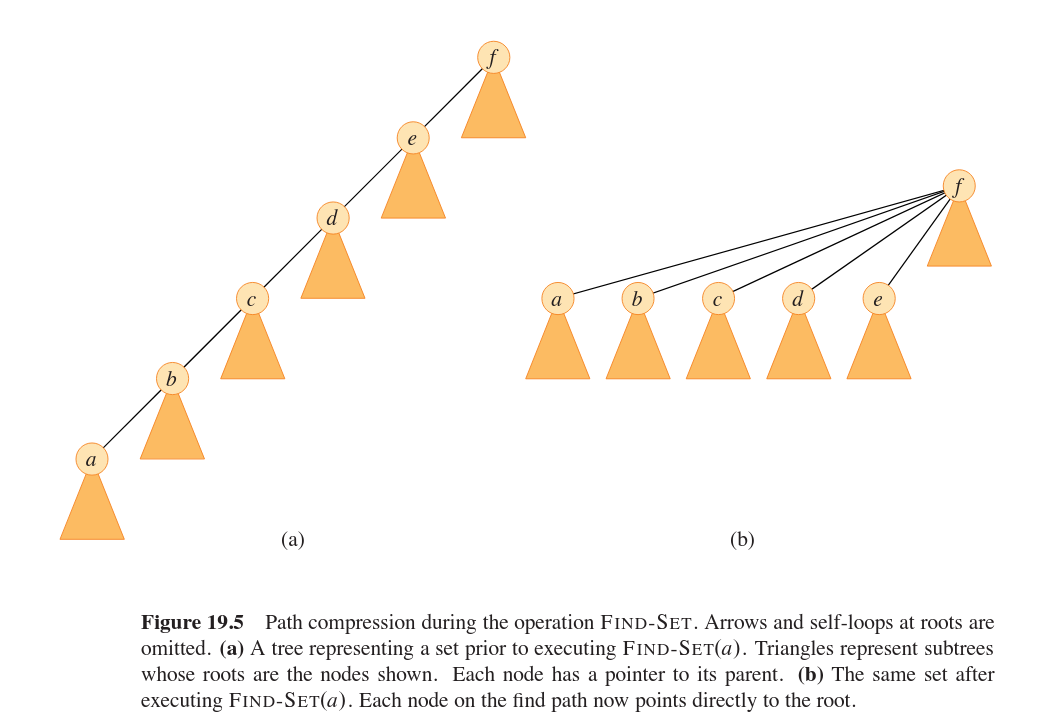
\includegraphics[width=\textwidth]{disjoint-set.png}
\end{figure}

We also ended up with an algorithm to do the exact operations we were interested in, namely:

\begin{enumerate}
    \item  \texttt{FIND-SET(x)}, to determine whether two nodes are in the same set, and
    \item \texttt{MAKE-SET(x)} and \texttt{UNION(x,y)}, to add new nodes and new edges to our sets
\end{enumerate}

This data structure and its associated algorithm are good if those are the two operations you want to do the most. However, sometimes we want to do some more general things with network-like data structure.

Commonly, we might want to know more than just whether two nodes are in the same set; we would like to understand how they are connected and what the structure of the connections is. 

In this case, we turn to some general \textit{graph algorithms}.

\section*{Graph Representations}

\subsection*{What is a Graph?}

Before we perform any sort of algorithms on our graphs, we need to be able to represent them computationally. 

Visually, a graph is a series of nodes or vertices connected by edges. We can draw this quite simply. 

Representing this in the computer is a bit more challenging. First, we have to turn our simple image into a more formal concept of what a graph is, mathematically. 

A graph $G$ is a collection of vertices, $V$, and a collection of edges, $E$, where each edge in $E$ connects exactly two vertices in $V$. Essentially, a graph can be represented by listing its vertices and its edges as follows:

\begin{verbatim}
    V = {1, 2, 3, 4, 5}
    E = {(1, 2), (1, 5), (2, 3), (2, 4), (2, 5), (3, 4), (4, 5)}
\end{verbatim}

\textbf{EXERCISE:} Draw the graph described above. 

\subsection*{How Do We Represent a Graph?}

Last class we discussed at length some representations of the graph of buildings at Lawrence University and their connections. While some of those ideas were incomplete for the exact task we wanted, they were very good for general graph algorithms. 

In general, there are two common representations for graphs: adjacency-list and adjacency-matrix.

\paragraph{Def.} The \textbf{adjacency-list representation} of a graph consists of an array, $A$, of $|V|$ lists. For each $u \in V$ the array $A[u]$ contains all vertices $v$ such that $(u, v) \in E$.

\paragraph{Def.} The \textbf{adjacency-matrix representation} of a graph arbitrarily numbers the vertices in $V$ and constructs a $|V| \times |V|$ matrix, called $A$, such that 

\begin{equation}
    a_{ij}=
    \begin{cases}
        1 & \text{if } (i, j) \in E\\
        0 & \text{otherwise}
    \end{cases}
\end{equation}

Construct the two different representations of the graph described above.

\textbf{QUESTION:} When might we want to use one representation over another? 

We might want to use an adjacency list when we are worried about the size of memory required, when our graph is very sparse, or when we are not so interested in doing a lookup to see if two nodes are connected.

Conversely, we might want to use an adjacency matrix when our graph is densely connected or when we would like to quickly look up a node connection. 

\textbf{DISCUSSION:} How might you change these representations from undirected to directed graphs? From unweighted to weighted? 

\subsection*{What Can We Do With Graphs?}

As mentioned earlier a common task for graphs is to find out the structure of the graph so that we can use this information to our advantage. After all, if the structure was unimportant, we could just store this information in a simple list. So usually we want to understand how the edges and vertices connect to one another. 

To do this, we will have to turn to some graph search algorithms. 

\section*{Search Algorithms for Graphs}

\subsection*{In-Class Exercise: Design an Algorithm}

What would you do in order to search a graph? 

Imagine I give you this graph. In words, describe how you might traverse the graph such that you visit every vertex at least once.

Your approach should also provide some information on the structure of the graph. This means you should either be able to:

\begin{enumerate}
    \item Provide some information about the shortest possible distance between some vertices in the graph, or
    \item Provide some information about the order of your search's traversal through the graph
\end{enumerate}

After you attempt this, we can turn to looking at common algorithms for these approaches.

\subsection*{Breadth-First Search}

The first algorithm we will look at is Breadth-First Search. This algorithm is commonly used when we are more interested in the first requirement: providing some information about distance between vertices. In particular, it's commonly used when we're interested in exploring the connections to a single \textit{source vertex} in the graph.

BFS explores the graph in ``waves'', starting with those vertices closest to the source, then two away, then three away, etc. 

BFS also uses ``colorings'' to keep track of the vertices it is exploring.

\begin{itemize}
    \item Vertices begin colored \texttt{white} and remain white until they are discovered in the search
    \item The first time a vertex is reached in the search, it is \textit{discovered} and becomes \texttt{grey}.
    \item Once all edges of a grey vertex have been explored, it becomes \texttt{black}.
\end{itemize}

Finally, BFS keeps track of the distance from the source vertex to each other vertex. 

Let's look at the pseudocode and then discuss some of the implementation details involved. 

\begin{figure}[h]
    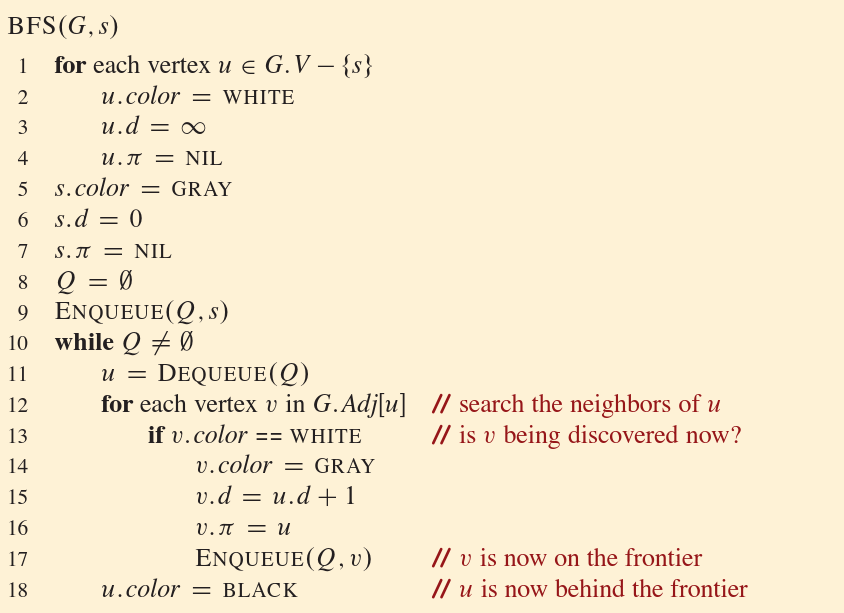
\includegraphics[width=\textwidth]{bfs-pseudocode.png}
\end{figure}

Notice that BFS maintains a \textit{queue} of the next vertices to be processed, and adds to the queue while there are still vertices to search. 

Here's a graphical representation of BFS.

\begin{figure}[h]
    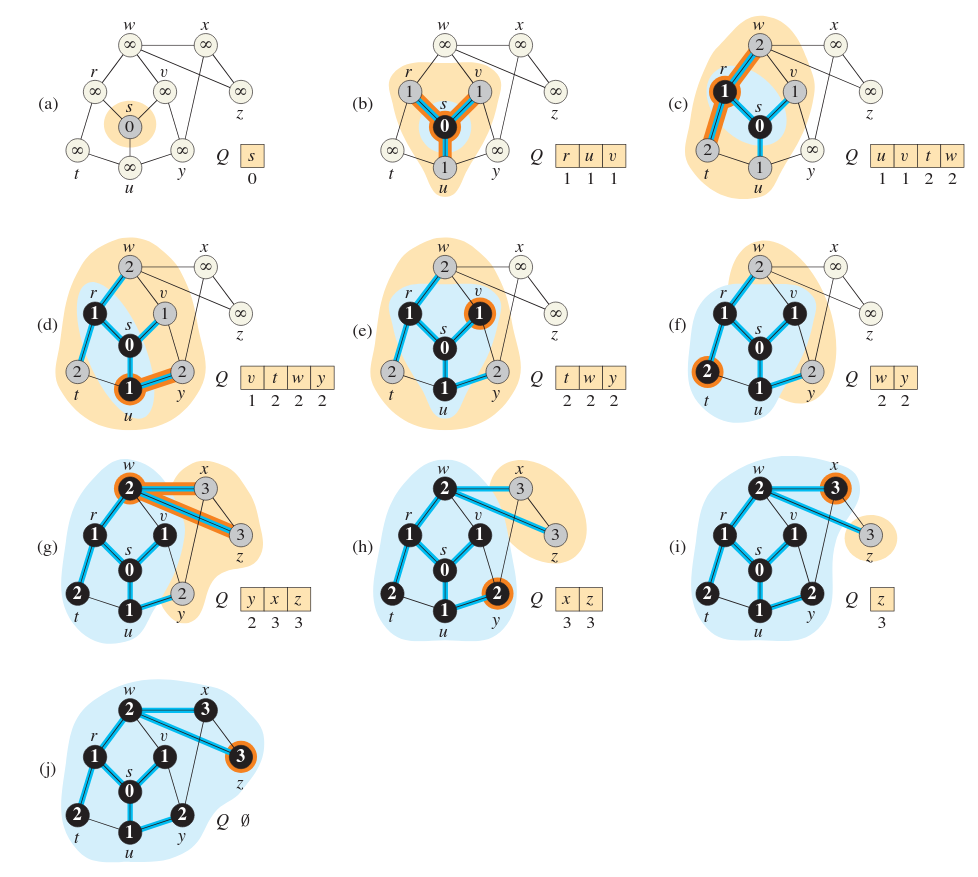
\includegraphics[width=\textwidth]{bfs.png}
\end{figure}

\textbf{QUESTION:} Where is the part in this algorithm where we move on to the next vertex to process? 

\textbf{QUESTION:} Will this algorithm visit every vertex? Will this algorithm visit every edge? Make an argument.

\subsection*{Depth-First Search}

An alternative to breadth-first search is depth-first search. This search is commonly used when we are less interested in finding shortest paths and more interested in doing an exhaustive search as part of some larger algorithm. (There are other reasons to use one over the other, but this is a common one.)

Depth-First Search (DFS) explores edges out of the most recent vertex that still has unexplored edges.

The coloring for DFS works in the same fashion as BFS. 

Another difference is what is tracked at each vertex. In DFS, we are not tracking distance from the source, but rather \textit{timestamps} for each vertex. Vertices are timestamped first when they are visited, and second when they are finished. 

\begin{figure}[h]
    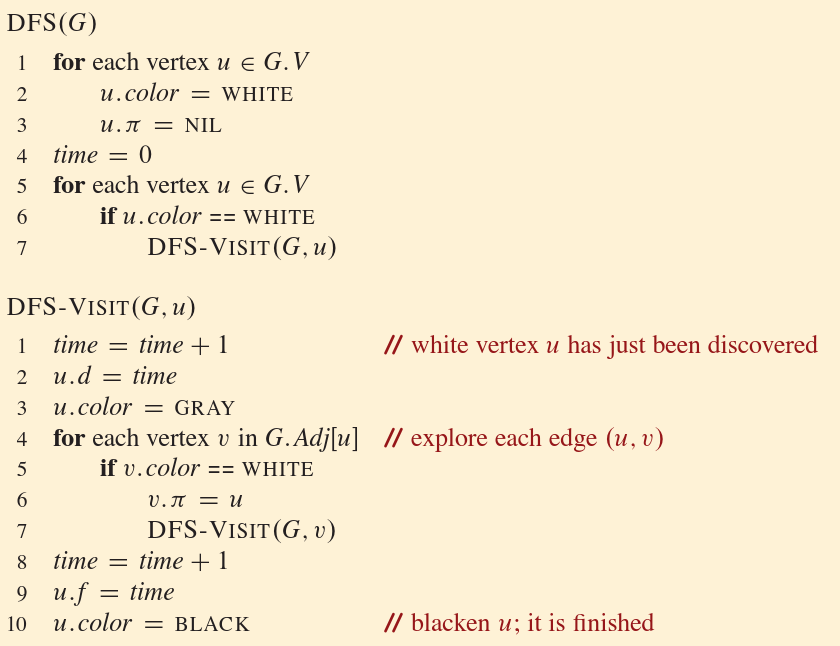
\includegraphics[width=\textwidth]{dfs-pseudocode.png}
\end{figure}

Notice here there is no queue to maintain. Why?

Here's a graphical representation of DFS.

\begin{figure}[h]
    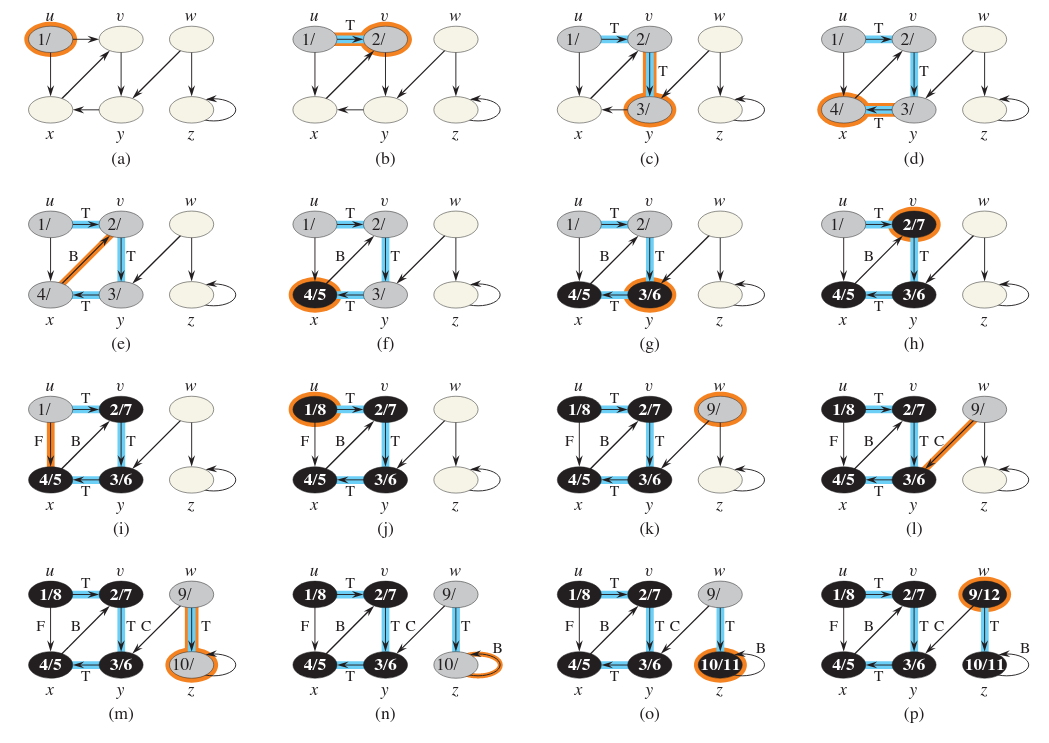
\includegraphics[width=\textwidth]{dfs.png}
\end{figure}

\textbf{QUESTION:} Looking at the image of DFS, where does the recursion `bottom out'? On which step?

\textbf{QUESTION:} Looking at the image of DFS, where does the recursion finish unfurling and move on to the next node? On which step? 

\section*{Applications of DFS: Toplogical Sort}

Here's an example of an algorithm that uses Depth-First Search as a subroutine for a larger problem. 

Suppose we have some directed acyclic graph (dag). Topological sorting ensures that we produce a linear ordering of all the vertices in the graph such that if $G$ contains an edge $(u, v)$, then $u$ appears before $v$ in the ordering. In general, topological sorts are helpful if we have some sort of dependency structure. 

The ``pseudocode'' for topological sort is very brief:

\begin{verbatim}
    TOPOLOGICAL-SORT(G):
        call DFS(G) to compute finish times
        as a vertex is finished, insert it ot the front of a linked list
        return the linked list
\end{verbatim}

This is an example of an algorithm that takes advantage of the depth property of DFS. 

\textbf{QUESTION:} Why use DFS here and not BFS? 

Since we can be sure that the first vertex finished is the deepest vertex from our start, we basicaly reverse-order the depth for topological sort. 

Here is the example the book gives of topological sorting, using clothing:

\begin{figure}[h]
    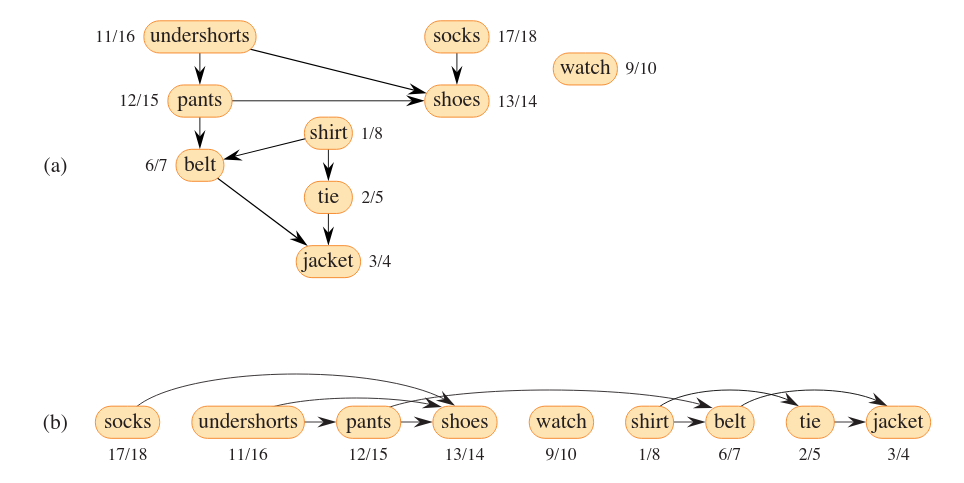
\includegraphics[width=\textwidth]{topo-sort.png}
\end{figure}

Can you come up with another example for which topological sort might be the right algorithm to use? 

\end{document}